

\fontsize{9}{12pt}\selectfont 

\vspace{-17pt}
\begin{center}
\textbf{\LARGE{Легко ли забить гвоздь?}} \\
\vskip 30pt
\textsf{\textbf{\large{А.КЛАВСЮК, Е.СОКОЛОВ}}}
    
\end{center}
\vspace{5pt}
\setlength{\columnsep}{20pt} 
\begin{multicols}{3}

\lettrine[lraise=0.2, nindent=1pt, lines=3]{\textbf{O}}{ДНАЖДЫ} в нашем классе разгорелся спор: можно ли с одного удара забить гвоздь? Мнения, как всегда, разделились. Одни доказывали, что никакой проблемы здесь нет. Другие, не менее горячо и аргументированно, что проблема есть
«силы не хватит». \par
А как же на самом деле обстоят дела? Всегда ли, размахнувшись посильнее, можно вогнать гвоздь в дерево с одного удара или есть случаи, когда одной силы недостаточно?

Давайте разберемся в этом вместе.

Итак, можно ли с одного удара забить гвоздь?\vskip 5mm

\noindent\rule{1\linewidth}{1pt} 
\textsf{{\Large{Результаты
\vspace{3pt}\\
экспериментов}}} 
\vspace{-5pt}\\
\noindent\rule{1\linewidth}{1pt} \\    
Прежде чем приступать к теоретичес ким рассуждениям, мы решили экспериментально установить, какую силу необходимо прикладывать к гвоздю для того, чтобы вдавливать его в дерево. Полученные нами результаты изображены на рисунке 1. Измерения проводились для двух сортов дерева: «мягкого» - ели и «твердого» - бука. В качестве эталонного гвоздя из всех собранных нами гвоздей (рис.2) мы выбрали обрезок длинного и толстого гвоздя -
длиной $l_0 = 50 \text{ мм}$ и радиусом поперечного сечения $R = 2 \text{ мм},$ -
который показался нам наиболее подходящим для подобных экспериментов. Вдавливание производилось с помощью пресса, позволяющего измерять прикладываемую силу.

В обоих случаях зависимость полу- чилась линейной:
$$ F(x) = F_0 + \frac{F_{max} - F_0}{l_0}x,$$
где $F_0$ равно 0,4 кН для ели и 1,1 кН для бука, $F_{max}$ равно, соответствен- но, 2,4 кН и 15,0 кН. Такую зависимость, на наш взгляд, и следовало ожидать.

При достаточно глубоком вдавли вании гвоздя $(x \gg R)$ в обжимающем гвоздь дереве можно выделить

\end{multicols}

%\hspace{-20mm}
%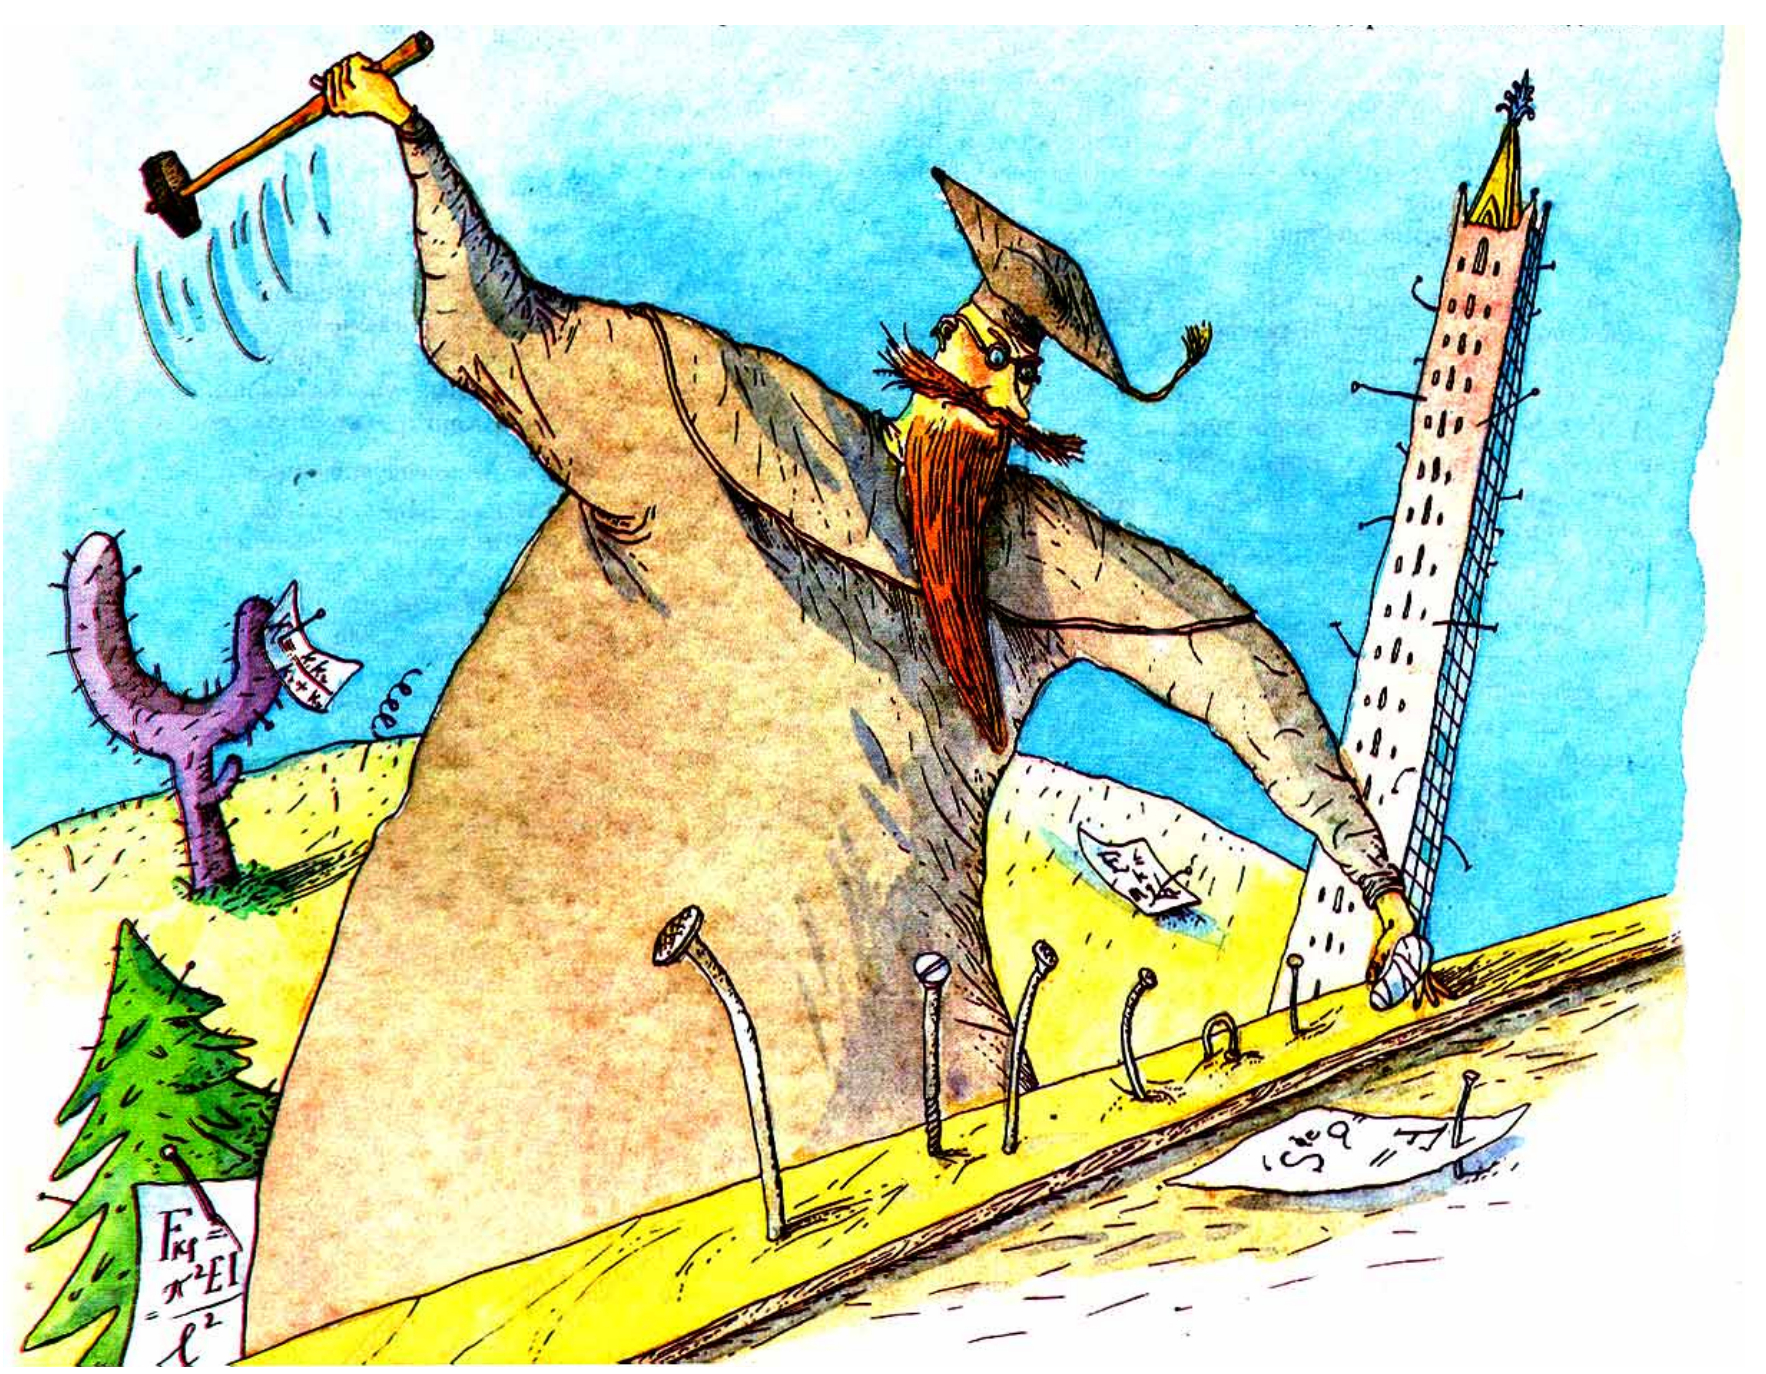
\includegraphics[width=210mm]{image.jpg} 
\AddToShipoutPictureBG*{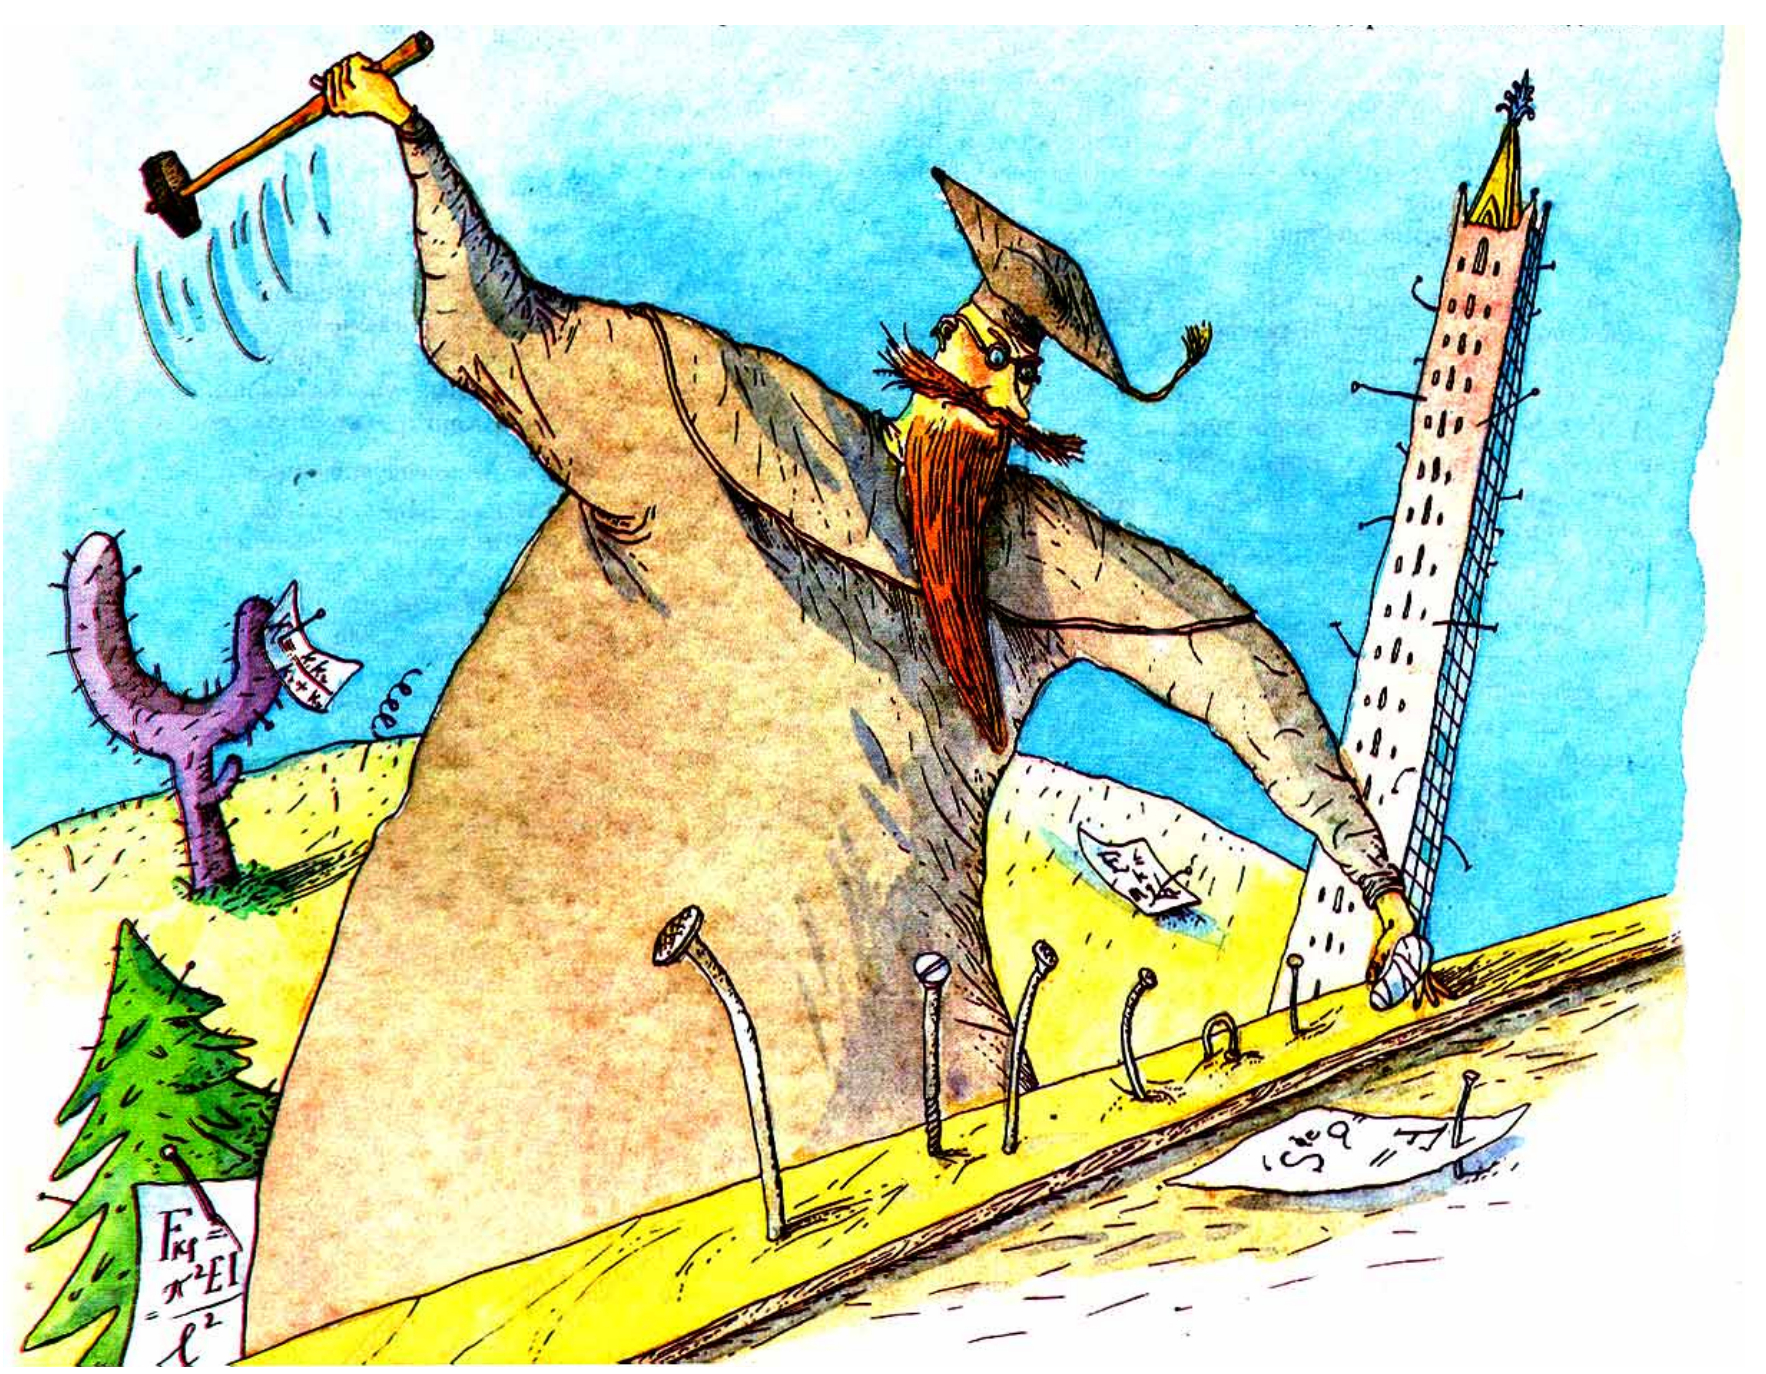
\includegraphics[width=\paperwidth]{image.jpg}};

\begin{textblock*}{5cm}(19.5cm,24cm) % Размер блока и координаты (x,y)
    \rotatebox{90}{\textbf{\textit{\textsf{Иллюстрация А.Балдина}}}}
\end{textblock*}
